\documentclass[11pt,a4paper]{article}
\usepackage{fontspec}
\setmainfont{TeX Gyre Pagella}
\newfontfamily\headfont{Inter}[UprightFont=*-ExtraBold,BoldFont=*-ExtraBold,Extension=.otf,Path=/usr/share/fonts/opentype/inter/]
\usepackage[a4paper,margin=2.3cm]{geometry}
\usepackage{graphicx,booktabs,float,caption,array,xcolor,longtable}
\usepackage{xurl}
\usepackage[hidelinks]{hyperref}
\usepackage{titlesec}
\usepackage[round]{natbib}
\usepackage{setspace}
\setstretch{1.05}
\renewcommand{\topfraction}{0.9}
\renewcommand{\bottomfraction}{0.8}
\renewcommand{\textfraction}{0.1}
\renewcommand{\floatpagefraction}{0.75}
\setlength{\parindent}{0pt}
\setlength{\parskip}{0.55em}
\titleformat{\section}{\headfont\Large}{\thesection}{0.8em}{}
\titleformat{\subsection}{\headfont\large}{\thesubsection}{0.8em}{}
\captionsetup{font=small,labelfont=bf}
\urlstyle{same}
\hypersetup{pdftitle={Ginnel, Snicket or Twitten?},pdfauthor={Tristan Hotham}}

\begin{document}
\begin{center}
{\Large\bfseries Ginnel, Snicket or Twitten?\par}
\vspace{0.4em}
{\large The regional words for an alley on the street signs of the United Kingdom, from OpenStreetMap\par}
\vspace{1.2em}
{\large Tristan Hotham\par}
\vspace{0.3em}
{\small Independent researcher\\
ORCID: 0000-0003-4931-9349\\
DOI: https://doi.org/10.5281/zenodo.24086513\par}
\vspace{0.8em}
2026
\end{center}

\begin{quote}
\small
\begin{center}\textbf{Abstract}\end{center}
English and Scots have dozens of words for a narrow passage between buildings, and their regional spread is a staple of dialect study. This paper asks how far those words reach the official record of street names. From 30,481 OpenStreetMap highways in the United Kingdom whose names contain an alley word, I keep names whose head word is one of 24 alley words, join pieces of the same alley, and remove false friends after reading every case of the ambiguous words (159 of 3,541 candidates, 4.5\%), leaving 3,382 named alleys. Regional words are tightly localised: 87.9\% of twittens are in Sussex, 98.4\% of lokes in Norfolk and Suffolk, all 45 chares in the North East of England, 96.9\% of opes in Devon, Cornwall and Dorset, and all 6 shuts in Shropshire. Scotland names its alleys with regional words, nearly all of them Scots (93.7\% of 1,294) far more often than England (28.1\% of 2,016), and London almost never does (2 of 375). The wynd, the commonest word, is now mostly a road name on new estates (77.8\% roads). The back-alley words of industrial towns (jigger, tenfoot, gully) hardly appear, a reminder that street names record official naming, not speech.

\textbf{Keywords:} dialect geography; street names; toponymy; alleys; Scots; OpenStreetMap
\end{quote}

\section{Introduction}
The narrow footway between houses has an unusually rich regional vocabulary in Britain: ginnel, snicket, twitten, twitchel, jitty, chare, wynd, close, vennel, pend, entry, loke, jigger, shut, ope, drang, tenfoot and more. The dialect dictionaries record many of them with a regional label \citep{wright1898}, and Scottish usage is covered by the Dictionary of the Scots Language \citep{dsl}. The Survey of English Dialects and the works drawn from it \citep{orton1962,upton1987,upton1994,upton1996} are the standard record of English dialect vocabulary, but I do not use their maps here. Most of that evidence is of speech. This paper asks a narrower question that a modern open map can answer: when an alley has an official or signposted name, which word does the name use, and where?

Street names are not speech. They are chosen by landowners, councils and, more and more, by developers, and many alleys have no name at all. But where the regional words do appear on signs, they are a durable and countable trace of local usage, and their absence is informative too. The result is a map of the alley words as the street plan records them, to set beside the dialect maps.

\section{Data}
\textbf{Highways.} OpenStreetMap ways in the United Kingdom with a \texttt{highway} tag and a name containing one of the alley words, or ending in Close, Row, Court, Yard, Wynd or Lane on footpath-type ways, queried with QLever \citep{bast2017}: 30,481 ways with the way identifier, highway type, name and the start of the geometry. OpenStreetMap is volunteered geographic information whose completeness varies from place to place \citep{haklay2010}. \textbf{Places.} Wikidata settlements with a population (CC0), of which towns and cities of 10,000 people or more are used to name the nearest town. \textbf{Counties.} ONS boundaries for counties and council areas.

\section{Method}
\textbf{Head words.} A name counts for a word only when the word is the head of the name: its last word, once trailing numbers, brackets and route notes after a dash are removed. Twitten Lane, Jetty Road, Chare Bank and Passage Road therefore do not count, while Ginnel No 7 and Twitten (Vernon Avenue to McWilliam Road) do. Spelling variants are grouped (ginnel, ginnell, jennel; twitchel, twitchell; jitty, gitty and, in the East Midlands only, jetty; vennel, vennal; drang, drangway). Close is counted only for footpath-type ways in Scotland, since in England a Close is usually a cul-de-sac; Row, Court, Yard and Lane are general words with other meanings and are left out. Table~\ref{tab:words} lists the words.

\textbf{Joining pieces.} OpenStreetMap often maps one alley as several ways. Ways of the same normalised name whose first points chain within 150 m are joined; ways of a road-type alley, or of a name with a specific element (Cornish Snicket), are joined within 600 m. Bare names on footpaths (Snicket, The Wynd) keep the 150 m rule because several separate paths can carry the same bare name. In all 3,256 ways were joined into others.

\textbf{False friends.} Every alley of the ambiguous words was read by eye, with its highway type, county and nearest town. Rules: a \textit{jetty} counts as a jitty only in Leicestershire, Northamptonshire, Rutland, Lincolnshire, Nottinghamshire, Derbyshire, Warwickshire and the West Midlands (elsewhere it is a pier or landing stage); a \textit{cut} counts only on a footway, pedestrian way, path or steps, never as New Cut, on a cycle trail or when any piece is a road (The Cut in Southwark is a street); \textit{steps} on a countryside path more than 3 km from a place of 3,000 people are hill paths. By hand (61 cases, \texttt{code/overrides.csv}): climbing gullies and mountain bike trails called Gully, Alley or Steps, cave passages under Mynydd Llangatwg, Tarr Steps (a clapper bridge) and other hill paths called Steps, racing pit lanes and farm tracks called Entry, an aqueduct (the Greenock Cut), peat cuttings, and a Welsh field name (Parc y Shut). Three misspelt or doubled names (\texttt{code/renames.csv}) were joined to the alley they belong to. 159 of 3,541 candidates were removed (4.5\%).

\textbf{Geography.} Each alley is placed at the mean of the first points of its ways and assigned to a county and to the nearest town of 10,000 people or more within 6 km (all of Greater London counts as London). For the overview map the UK is divided into hexagons 20 km across on the British National Grid; a hexagon is coloured by its commonest regional word when it has at least three alleys with a regional word.

\begin{small}\begin{longtable}{p{2.0cm}p{2.9cm}p{4.1cm}rrp{3.1cm}}\caption{The alley words: spellings counted, the region where the word is usually reported (context, not a result), named alleys in the data, share that are footpaths (\%), and the county with most.}\label{tab:words}\\\toprule Word & Spellings & Usually & Alleys & Path & Top county\\\midrule\endhead
ginnel & ginnel, ginnell, gennel, jennel, jinnel & Lancashire, Greater Manchester and West Yorkshire & 26 & 88 & West Yorkshire (35\%)\\
snicket & snicket, snickets, snickelway & Yorkshire and Humberside & 18 & 100 & West Yorkshire (39\%)\\
twitten & twitten, twittens & Sussex & 33 & 79 & West Sussex (45\%)\\
twitchel & twitchel, twitchell, twitchill, twitch & Nottinghamshire and the East Midlands, also parts of Essex and Hertfordshire & 8 & 38 & Nottinghamshire (38\%)\\
jitty or gitty & jitty, gitty, jetty & the East Midlands: Leicestershire, Derbyshire, Nottinghamshire, Northamptonshire & 32 & 84 & Leicestershire (25\%)\\
chare & chare, chares & Newcastle, Durham and the North East & 45 & 38 & Tyne and Wear (44\%)\\
wynd & wynd, wynds & Scotland and the North East of England & 957 & 22 & Fife (15\%)\\
vennel & vennel, vennal, vennels & Scotland and the North East of England & 50 & 54 & Perth and Kinross (14\%)\\
close (Scotland) & close & Scotland: the narrow entries off the old high streets & 253 & 100 & City of Edinburgh (34\%)\\
pend & pend & Scotland: a passage through a building & 24 & 54 & Dundee City (21\%)\\
entry & entry, entries & Merseyside, Birmingham and the West Midlands, Lancashire, Belfast & 81 & 72 & City of Edinburgh (15\%)\\
loke & loke, lokes & Norfolk and Suffolk & 188 & 36 & Norfolk (93\%)\\
jigger & jigger, jiggers & Liverpool & 0 & & \\
shut & shut, shuts & Shrewsbury and Shropshire & 6 & 100 & Shropshire (100\%)\\
ope & ope, opes & Plymouth and Devon, also Cornwall & 32 & 59 & Devon (53\%)\\
drang or drong & drang, drong, drangway & Devon and the West of England & 11 & 73 & Cornwall (27\%)\\
lonnen & lonnen, lonning, lonnin & the North East and Cumbria (a lane) & 24 & 38 & Tyne and Wear (46\%)\\
gully & gully, gulley, gullies & Birmingham and the Black Country & 6 & 100 & Bristol (50\%)\\
tenfoot & tenfoot & Hull, the East Riding and north Lincolnshire & 1 & 100 & East Riding of Yorkshire (100\%)\\
alley & alley, alleyway, alleys & standard English & 484 & 88 & Greater London (21\%)\\
passage & passage & standard English & 671 & 88 & Greater London (36\%)\\
steps & steps & standard English, often steep towns & 393 & 97 & Devon (9\%)\\
backway & backway, backways & standard English: a way round the back & 11 & 55 & Devon (18\%)\\
cut & cut & standard English: a short cut & 26 & 100 & Durham (27\%)\\
slype & slype & a passage by a cathedral or abbey (an architectural word) & 2 & 0 & Hertfordshire (100\%)\\
\bottomrule\end{longtable}\end{small}

\section{Results}
\subsection{Scotland and England}
The data hold 3,382 named alleys: 1,795 with a regional word and 1,587 with a general one (alley, passage, steps, backway, cut). The split differs sharply by nation: 93.7\% of Scotland's 1,294 named alleys carry a regional word, against 28.1\% of England's 2,016, 8.9\% of Wales's 56 and 75.0\% of Northern Ireland's 16. Greater London has the most named alleys of any town (375), but only 2 use a regional word; the rest are 244 passages, 102 alleys and steps. Of 121 hexagons with at least three regional names, the wynd leads in 61 (Figure~\ref{fig:hex}).

\begin{figure}[tbp]\centering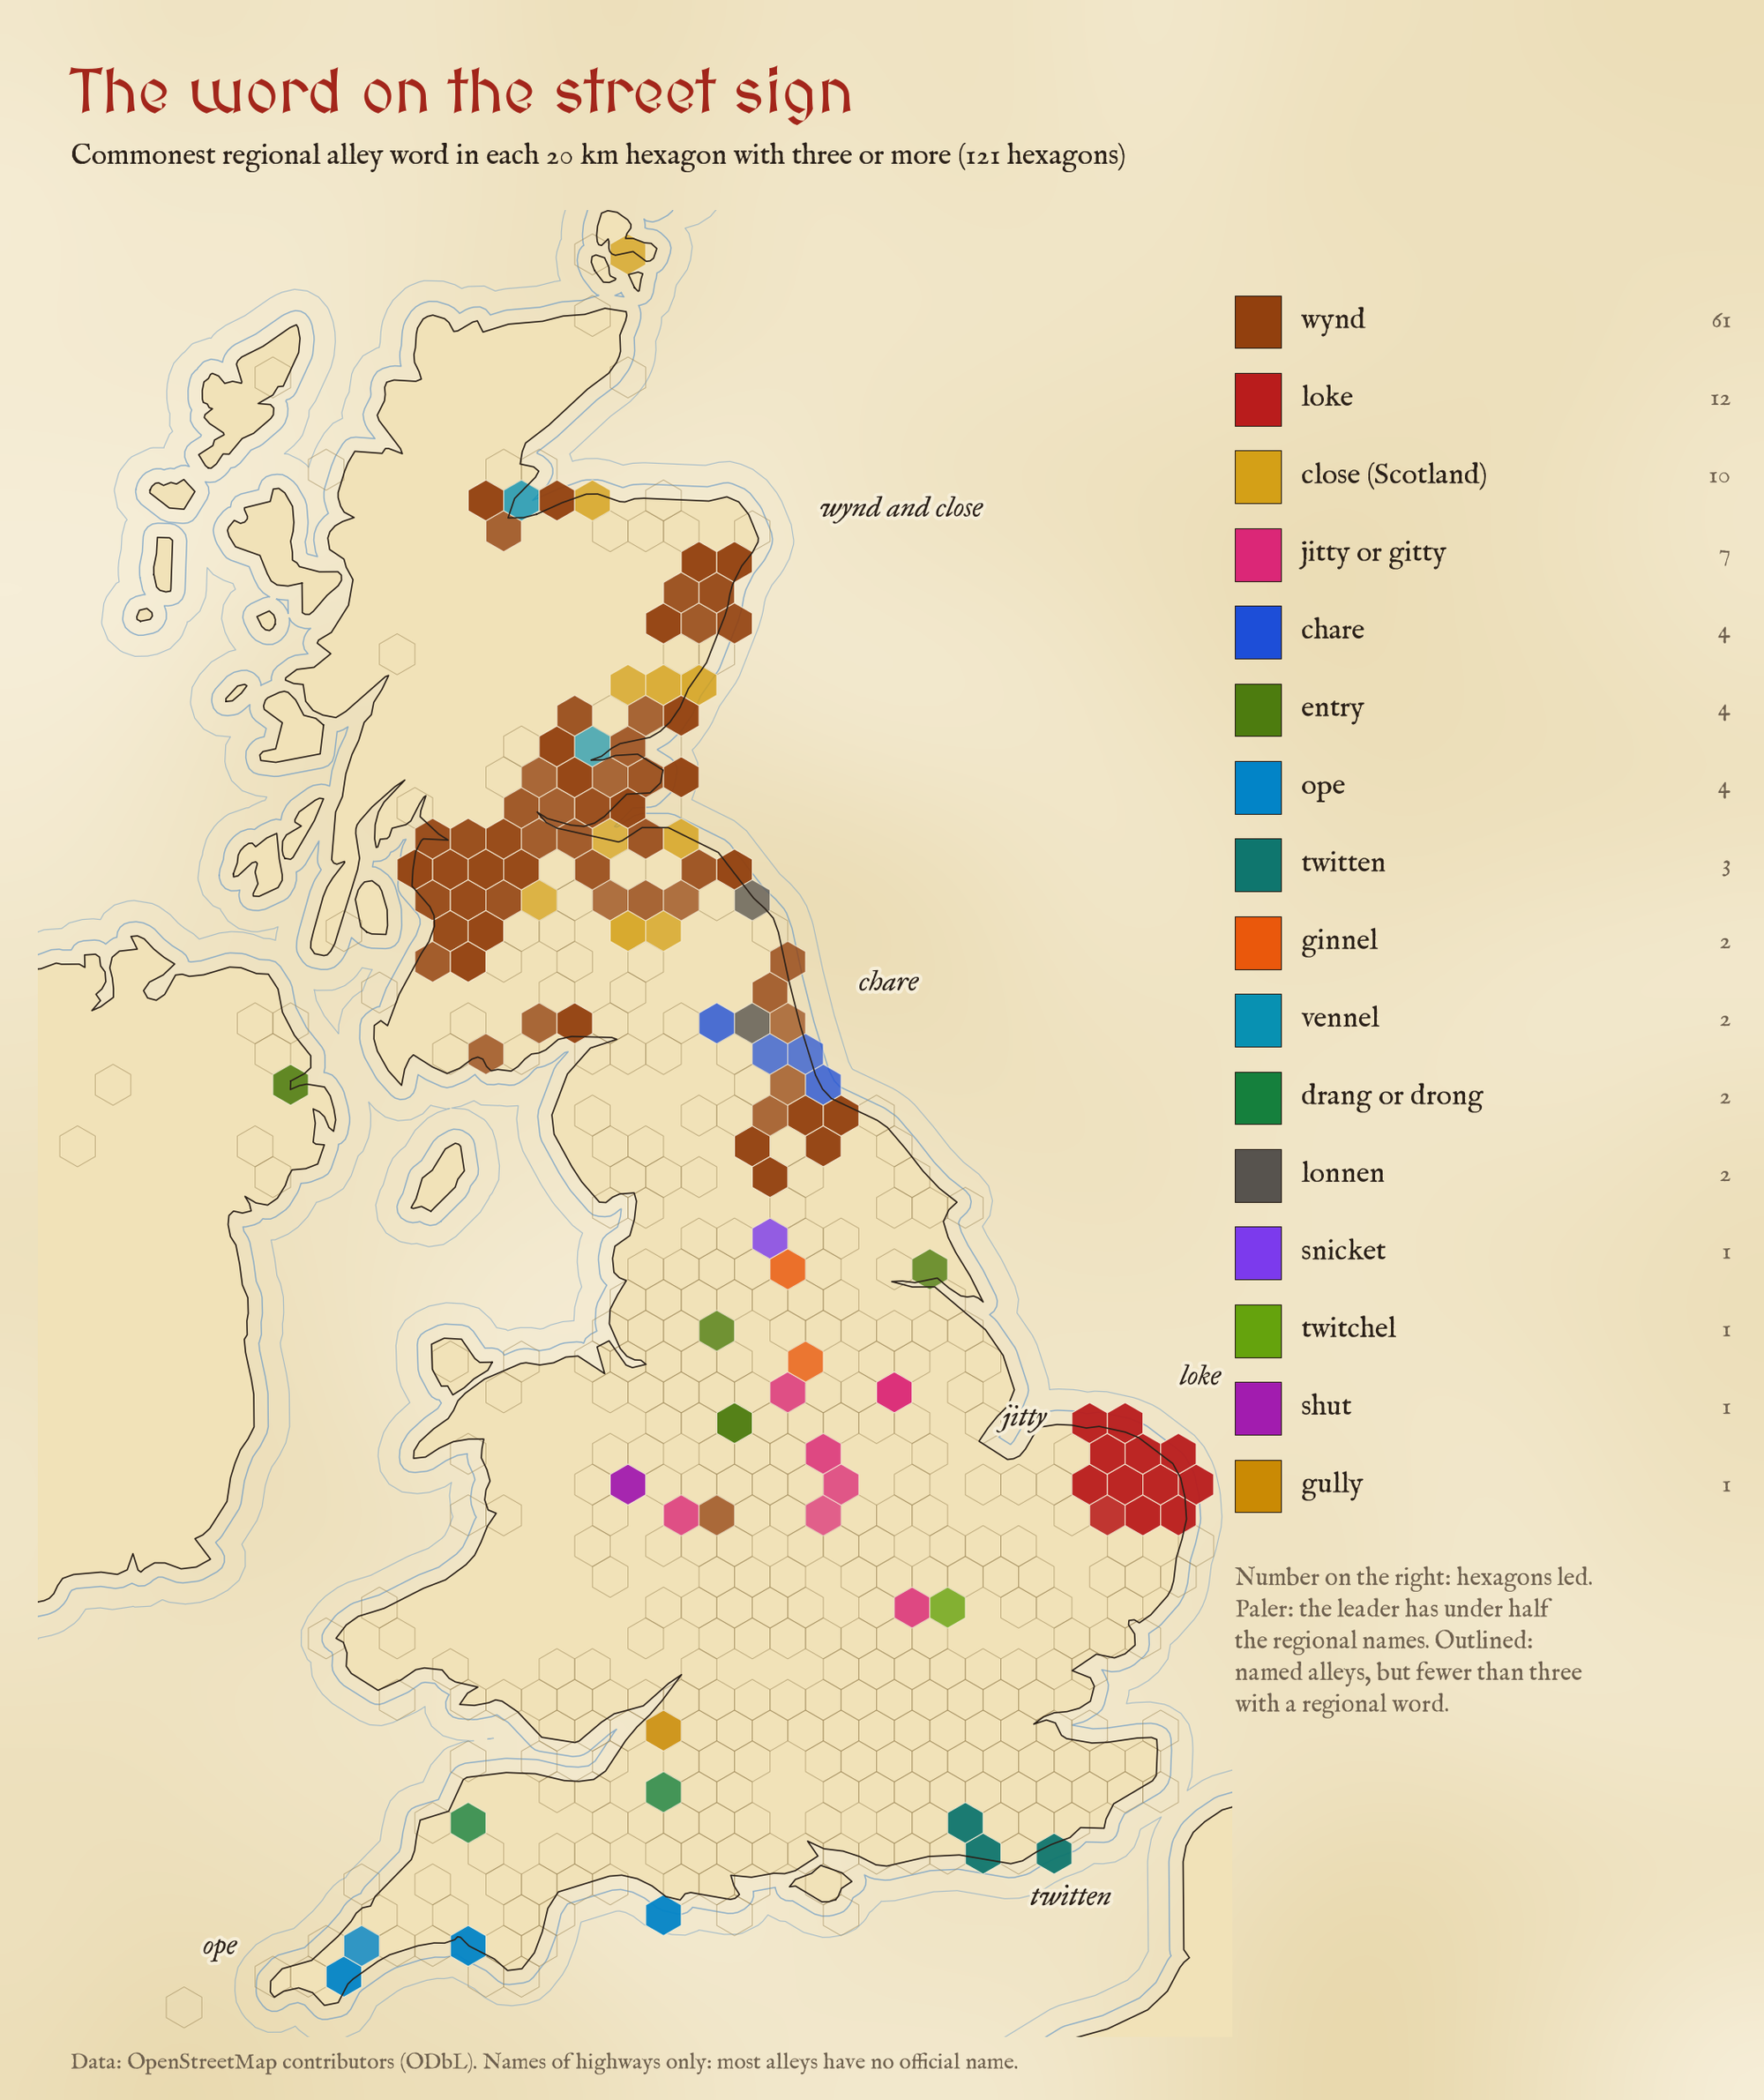
\includegraphics[width=0.86\textwidth]{f_hexmap.png}
\caption{The commonest regional alley word in each 20 km hexagon with at least three named alleys that use one.}\label{fig:hex}\end{figure}

The wynd (957 alleys, 850 in Scotland and 91 in the North East of England and North Yorkshire) is the commonest word but has changed character: only 22.2\% are footpaths, and most are roads on recent housing estates in Fife, Lanarkshire and Ayrshire. The Scottish close is the opposite: as counted here it is always a footpath, and 85 of the 253 (33.6\%) are in the City of Edinburgh, with 18 in Elgin. Vennels (50) are commonest in Perth, and pends (24) in Dundee and Edinburgh. Entries (81) are spread more widely: Edinburgh (12), Belfast (6, the entries off High Street and Ann Street), Cheadle in Staffordshire, the Borders and Perthshire.

\subsection{Regional words in England}
Where English regional words reach the street sign they cluster tightly (Figure~\ref{fig:small}). 29 of 33 twittens (87.9\%) are in East or West Sussex; 185 of 188 lokes (98.4\%) in Norfolk or Suffolk, 17 of them near North Walsham; all 45 chares in Tyne and Wear, Durham and Northumberland, 15 in Newcastle; 31 of 32 opes (96.9\%) in Devon, Cornwall and Dorset, 15 in Plymouth; all 6 shuts in Shropshire. Jitties (32) are 78.1\% East Midland, with an outlying group in the Ironbridge Gorge; ginnels (26) are 88.5\% in the northern counties; lonnens, a Northumbrian word for a lane, are 95.8\% in the North East and Cumbria; drangs (11) are in the South West.

\begin{figure}[tbp]\centering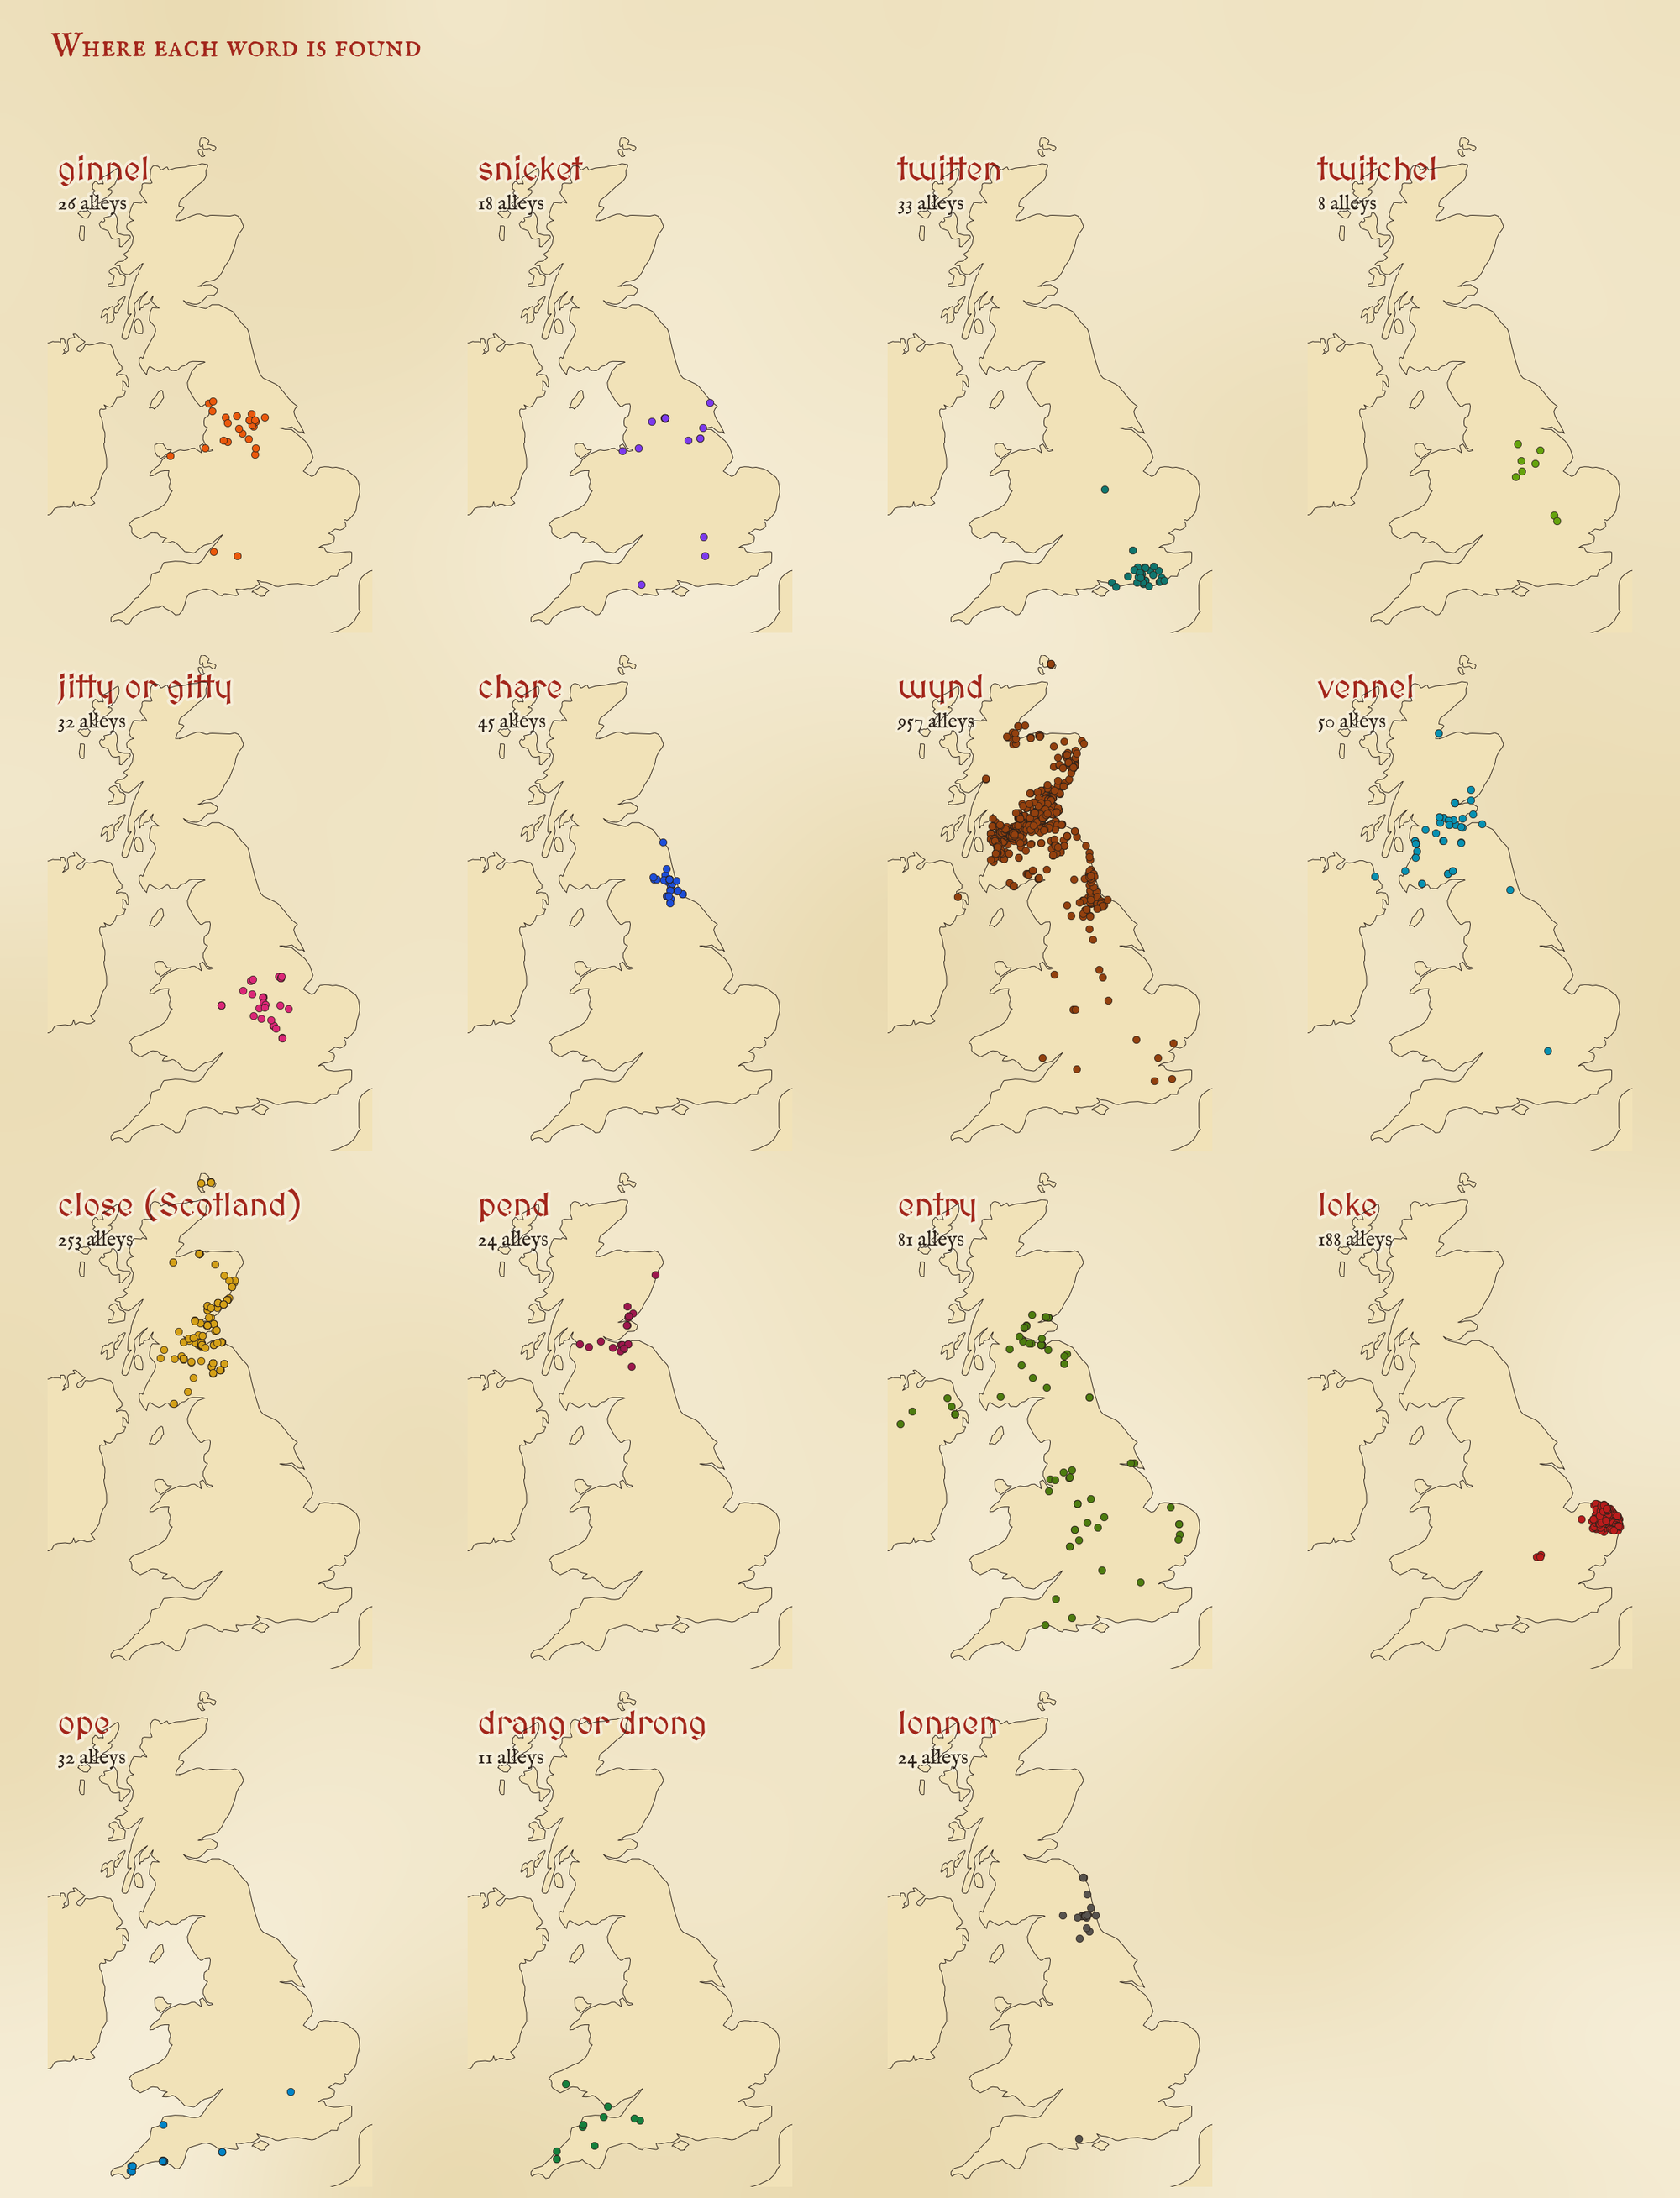
\includegraphics[width=\textwidth]{f_small.png}
\caption{Every named alley with each regional word that has at least seven.}\label{fig:small}\end{figure}

These are the regions the dialect dictionaries give for the words \citep{wright1898,dsl}, so where the official names exist they agree with the record of speech. I have not compared them map for map with the Survey of English Dialects or the atlases drawn from it. The agreement is a check on the method rather than a new finding. The new part is how few of the words reach the sign at all, and where they do not.

\subsection{Where the words meet}
In Yorkshire the street signs have 14 ginnels and 10 snickets. The ginnels are in and around Leeds, Huddersfield, Harrogate, Skipton and Sheffield; 7 of the snickets are footpaths named simply Snicket around Burley in Wharfedale, 9.1 km from the nearest ginnel at Yeadon (Figure~\ref{fig:meet}). York, where the word \textit{snickelway} was coined for the city's lanes \citep{jones1983}, has no alley named snicket or snickelway. On Tyneside, chares (the Quayside lanes of Newcastle and the old streets of Durham towns) meet lonnens and wynds; in Sussex the twittens are a country and small-town word, while Brighton and Hastings name most of their alleys passages or steps.

\begin{figure}[tbp]\centering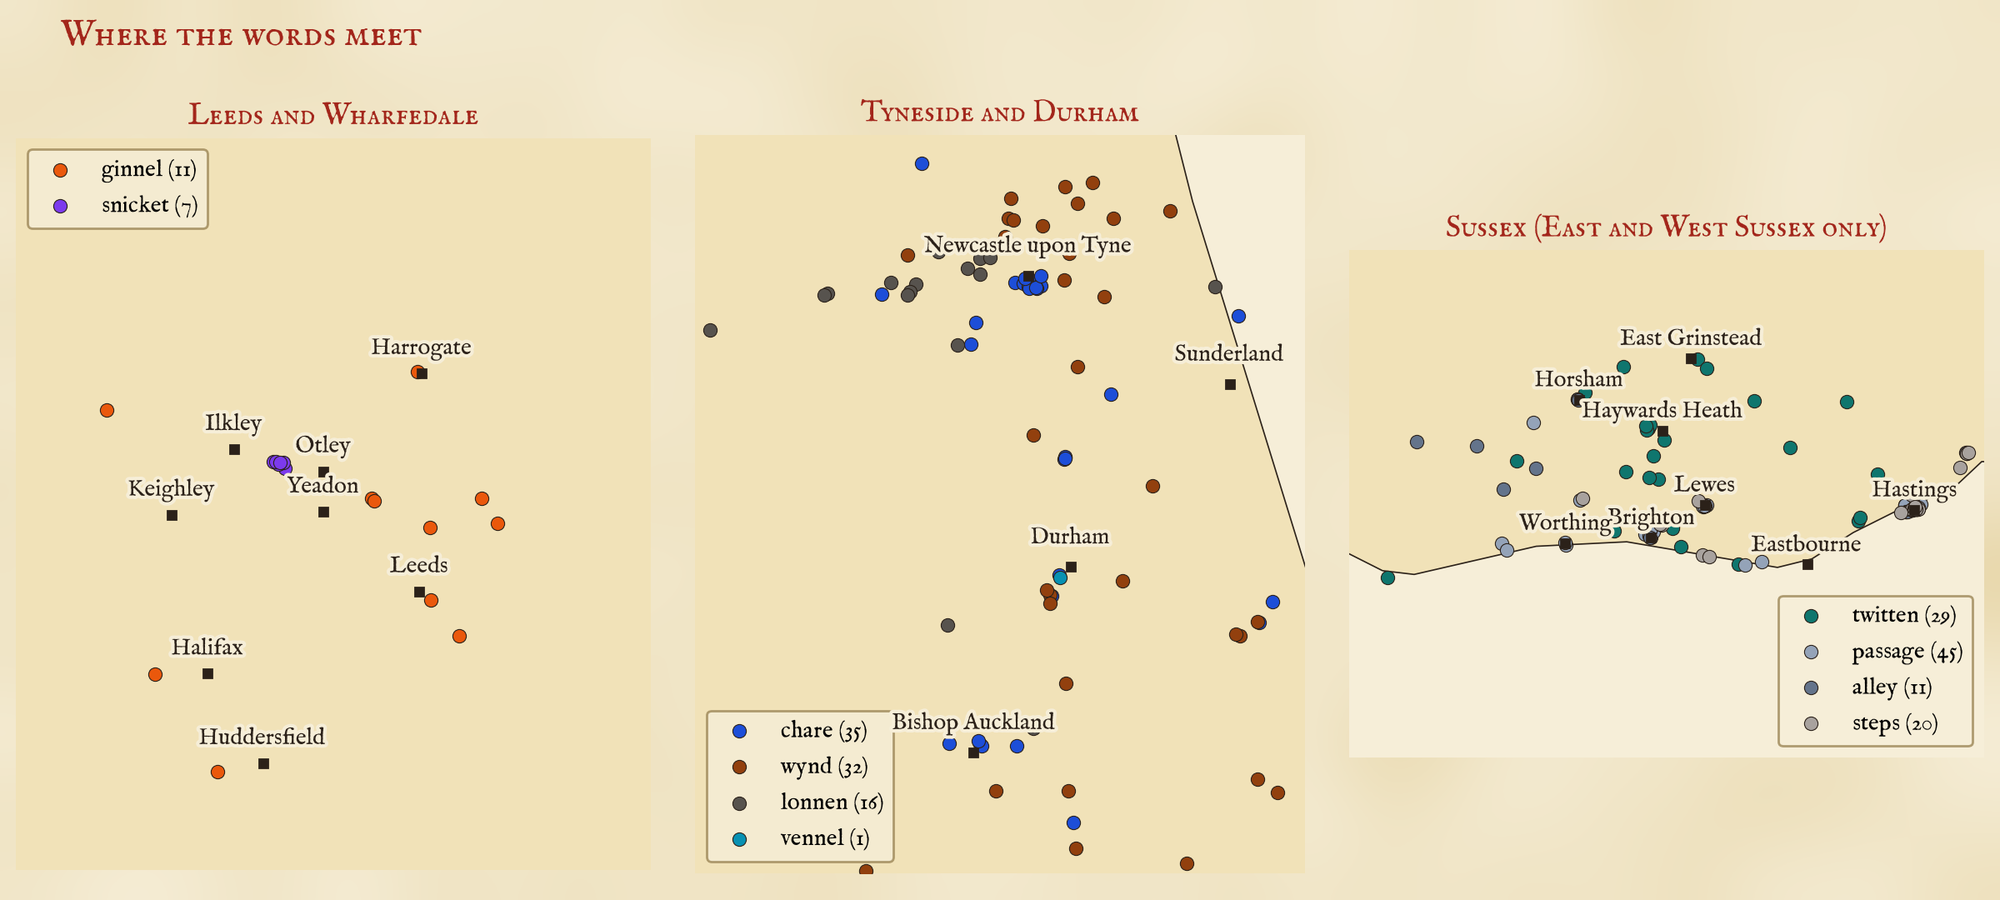
\includegraphics[width=\textwidth]{f_meet.png}
\caption{Where words meet: Leeds and Wharfedale, Tyneside and Durham, and Sussex.}\label{fig:meet}\end{figure}

\subsection{Towns}
The most named alleys are in London (375), Edinburgh (127) and Hastings (38) (Figure~\ref{fig:towns}). Edinburgh has the most with a regional word (116) and the most different words (7); then come Kirkcaldy, Dundee, Elgin and Aberdeen.

\begin{figure}[tbp]\centering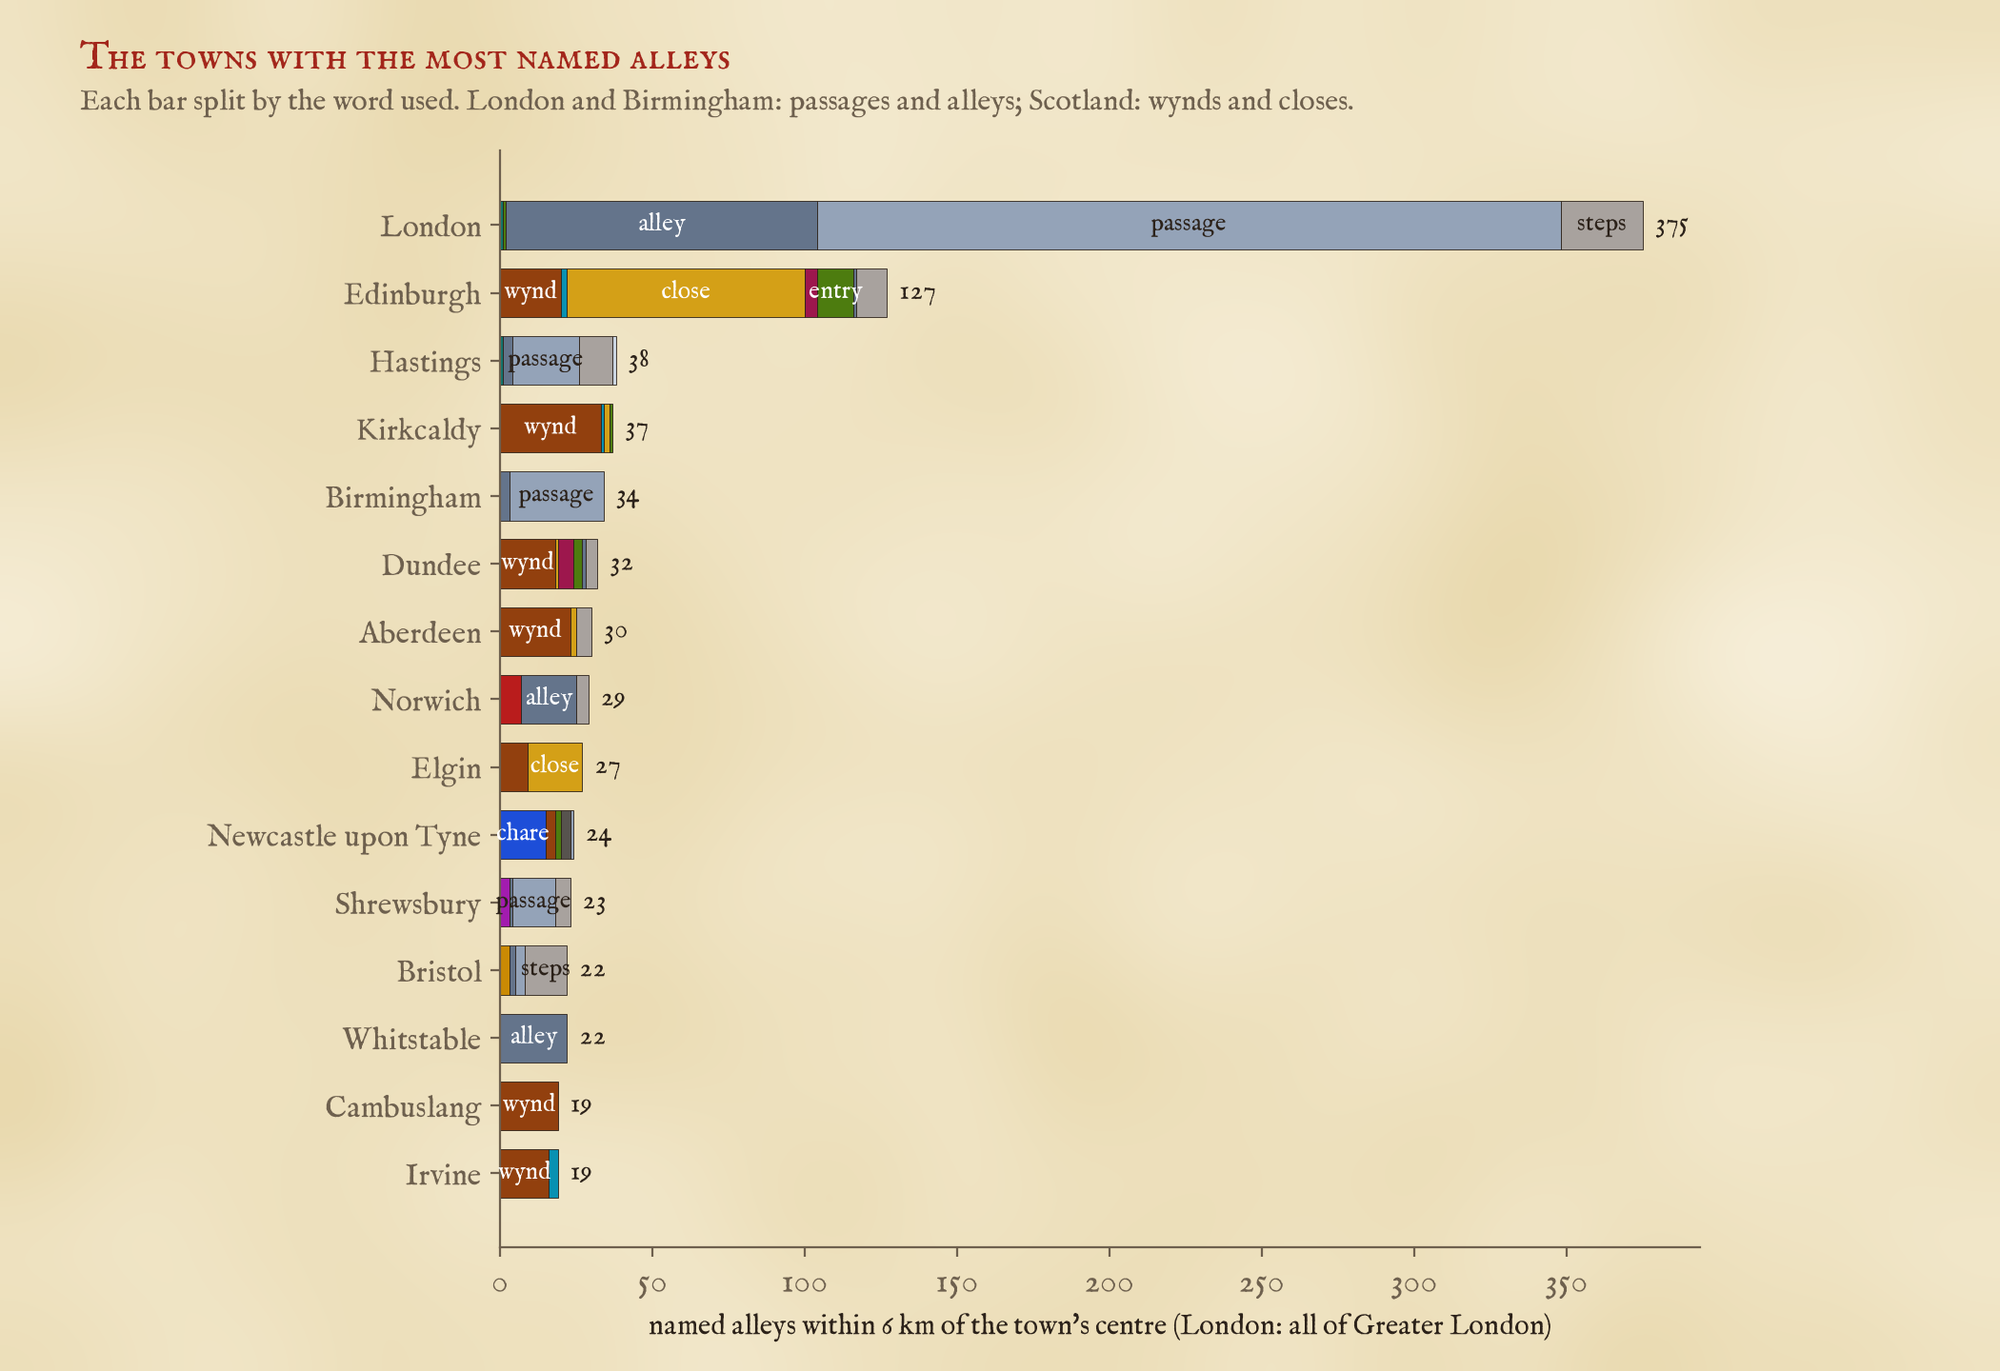
\includegraphics[width=0.92\textwidth]{f_towns.png}
\caption{The towns with the most named alleys within 6 km of the centre (Greater London as one), by word.}\label{fig:towns}\end{figure}

\subsection{The words that do not reach the sign}
Some of the best known alley words barely appear. There is no alley named jigger in Liverpool or anywhere else, although jigger was one of the search words (the only Jigger names in the data are a Jigger Grove and a Jigger Gardens far from Merseyside, where the word is not the head), 1 tenfoot (near Hull), and no gully in Birmingham; half of the 6 gullies kept are in Bristol. These words belong to the back alleys of nineteenth-century terraces, which were rarely named. The names that do survive belong to two other kinds of place: the older lanes of town centres (chares, closes, opes, shuts, lokes) and the street names of new estates, where a regional word is chosen for local colour (wynd, and some twittens, lokes and chares). Figure~\ref{fig:words} shows how many alleys carry each word and how many are footpaths.

\begin{figure}[tbp]\centering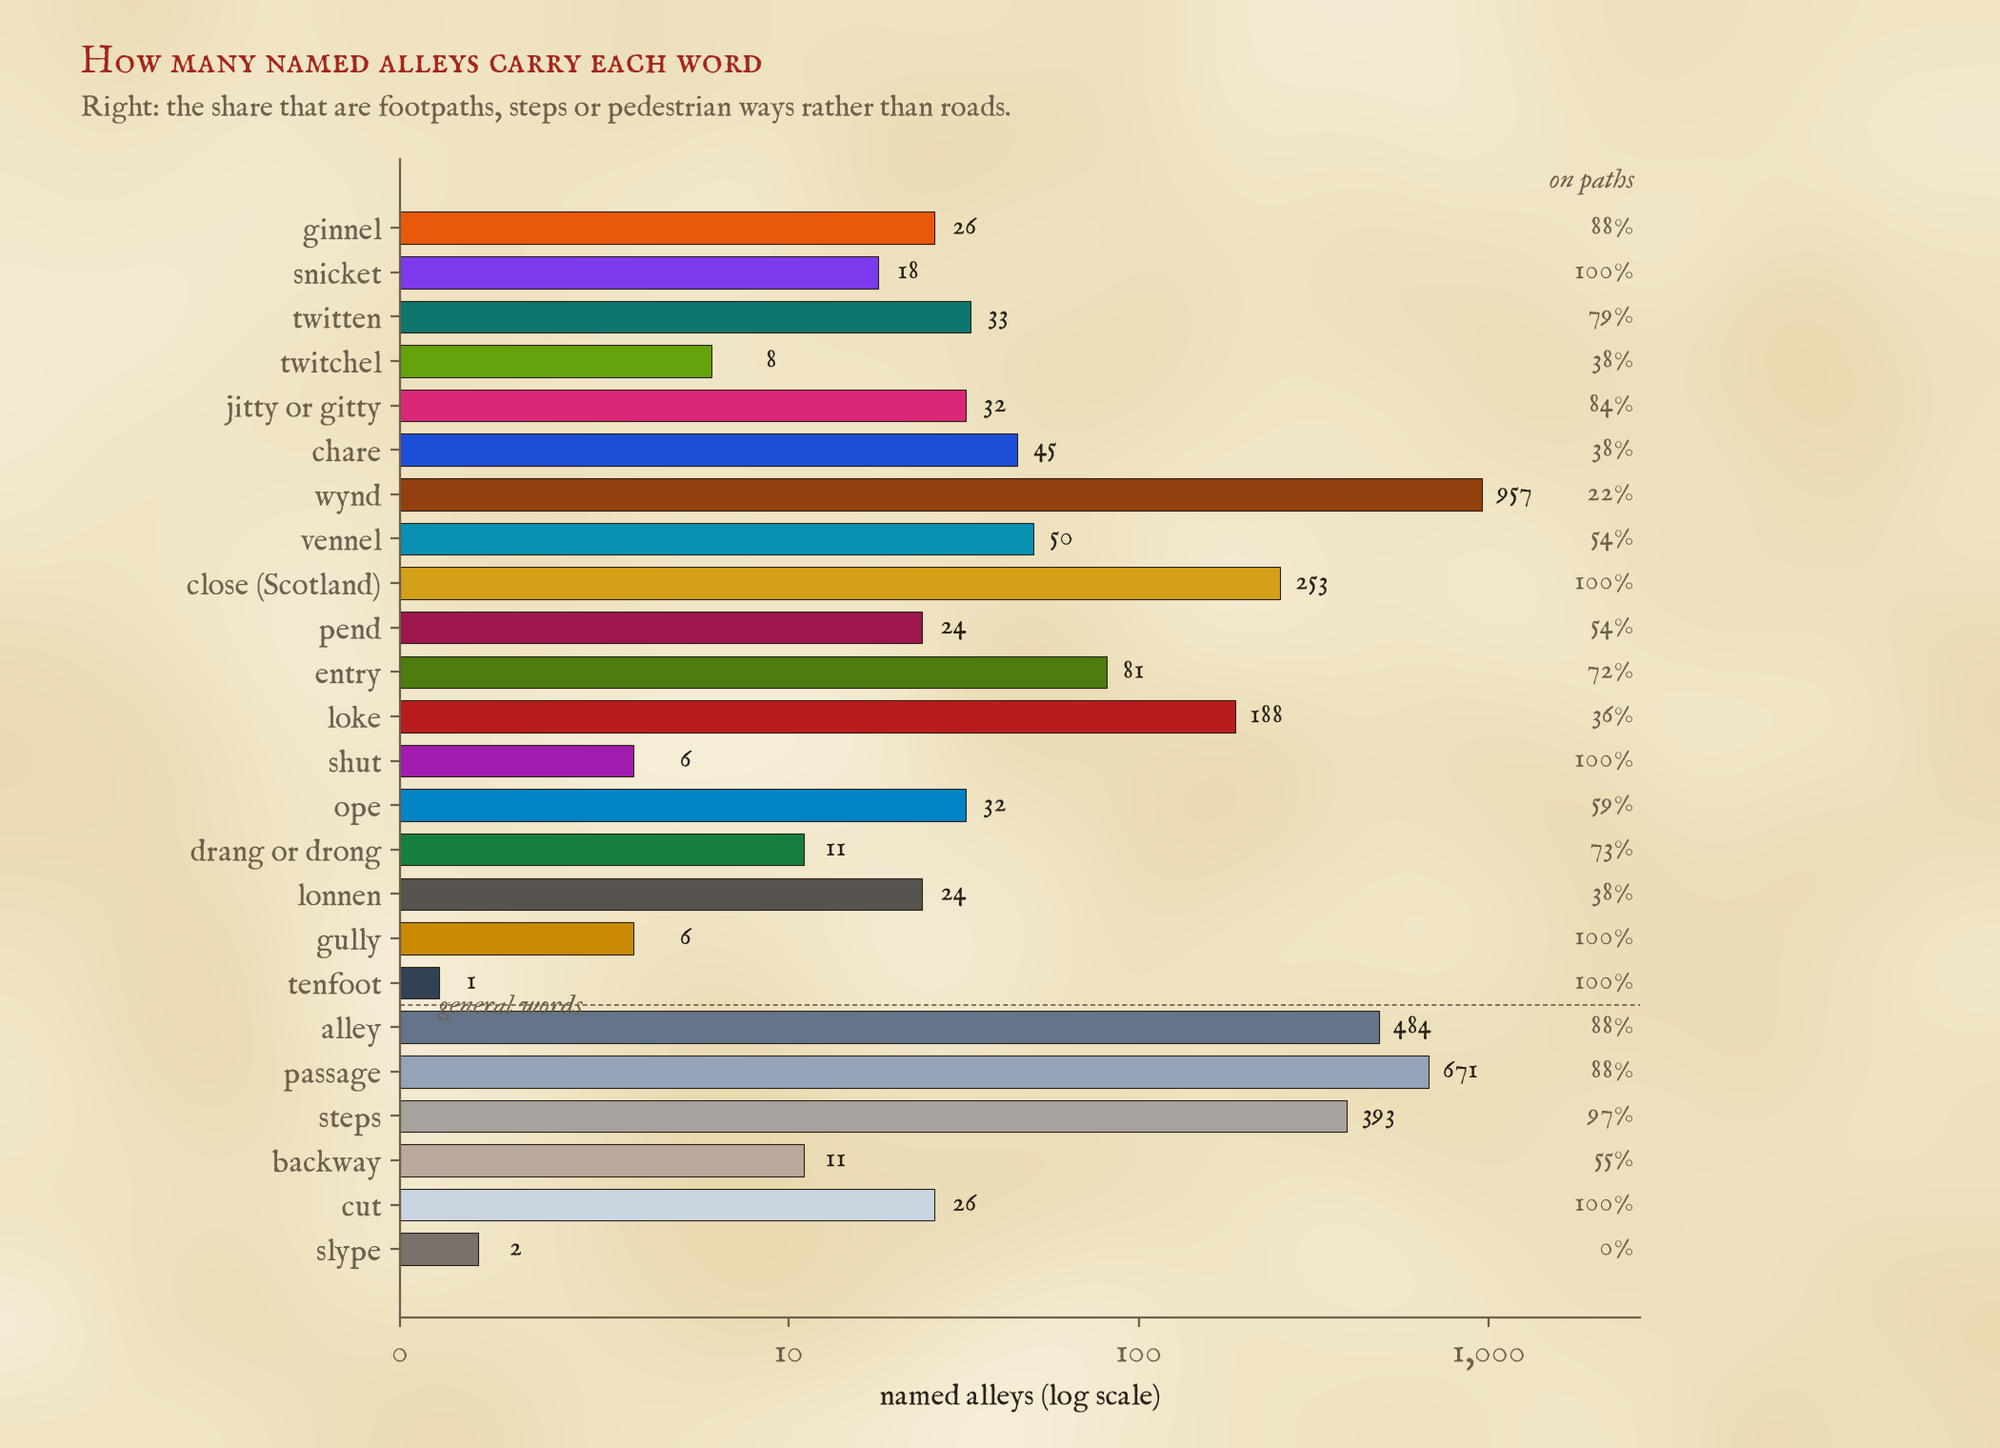
\includegraphics[width=0.92\textwidth]{f_words.png}
\caption{Named alleys by word (log scale) and the share that are footpaths, steps or pedestrian ways.}\label{fig:words}\end{figure}

\section{Limitations}
Street names are official names. They show where a word was thought right for a sign, not how people speak, and the dialect sources are cited for context only; no comparison here re-reads their maps. Most alleys have no name in OpenStreetMap, and naming varies with the mappers of each area \citep{haklay2010}: a cluster of paths named Snicket near Burley in Wharfedale may reflect one parish's signs or one mapper's habit. Counts for the rarer words are small. The first point of each way is used, so an alley's position is approximate, and joining by distance can merge two alleys of one name or leave one alley in two pieces. The false-friend rules were checked by eye for the ambiguous words, but the large groups of unambiguous words (wynd, passage, alley) were checked by rule and spot reading only. Close is counted only in Scotland and only on footpaths, which undercounts closes that are mapped as service roads; the query itself fetched Close only on footpath-type ways. More generally the query matched only the listed words, so a word left off the list (eightfoot, for example) cannot appear, and an absence such as the jigger means absent among names containing the word, not absent from the street. Each alley goes to the nearest town point, so an alley on the edge of a city can be counted to a neighbouring town (one Plymouth ope is counted to Saltash).

\section{Conclusion}
On the street signs of the United Kingdom, the regional words for an alley are real but rare outside Scotland. Where they appear they sit exactly in their home regions: twitten in Sussex, loke in Norfolk, chare in the North East, ope around Plymouth, shut in Shrewsbury, jitty in the East Midlands. Scotland names its narrow ways in Scots, London almost never in anything but standard English, and the back-alley words of the industrial north and Midlands remain spoken rather than signed.

\section*{Data and code availability}
The interactive map is at \url{https://maps.tristanhotham.com/alleyway-words/}. Code, the rules and hand decisions, and the derived tables are at \url{https://github.com/Tristan-Hotham/alleyway-words} and archived with this paper at https://doi.org/10.5281/zenodo.24086513. The alley tables are derived from OpenStreetMap (\copyright{} OpenStreetMap contributors) and released under the Open Database Licence; Wikidata is CC0; county boundaries from the ONS (Open Government Licence v3.0); text and figures CC BY 4.0; code MIT.

\section*{AI statement}
I wrote the text, with drafting and editing assistance from Claude (Anthropic), which also helped prepare the analysis code. I reviewed and checked all text and results.

\begin{thebibliography}{10}
\bibitem[Bast and Buchhold(2017)]{bast2017} Bast, H. and Buchhold, B. (2017) QLever: a query engine for efficient SPARQL+Text search. \textit{Proceedings of the 2017 ACM Conference on Information and Knowledge Management (CIKM)}, 647 to 656.
\bibitem[Dictionary of the Scots Language(n.d.)]{dsl} Dictionary of the Scots Language. Edinburgh: Scottish Language Dictionaries. Online at dsl.ac.uk.
\bibitem[Haklay(2010)]{haklay2010} Haklay, M. (2010) How good is volunteered geographical information? A comparative study of OpenStreetMap and Ordnance Survey datasets. \textit{Environment and Planning B: Planning and Design} 37(4), 682 to 703.
\bibitem[Jones(1983)]{jones1983} Jones, M. W. (1983) \textit{A Walk Around the Snickelways of York}. York: the author.
\bibitem[Orton and Dieth(1962 to 1971)]{orton1962} Orton, H. and Dieth, E. (eds) (1962 to 1971) \textit{Survey of English Dialects: The Basic Material}. Leeds: E. J. Arnold.
\bibitem[Upton et al.(1987)]{upton1987} Upton, C., Sanderson, S. and Widdowson, J. (1987) \textit{Word Maps: A Dialect Atlas of England}. London: Croom Helm.
\bibitem[Upton et al.(1994)]{upton1994} Upton, C., Parry, D. and Widdowson, J. D. A. (1994) \textit{Survey of English Dialects: The Dictionary and Grammar}. London: Routledge.
\bibitem[Upton and Widdowson(1996)]{upton1996} Upton, C. and Widdowson, J. D. A. (1996) \textit{An Atlas of English Dialects}. Oxford: Oxford University Press.
\bibitem[Wright(1898 to 1905)]{wright1898} Wright, J. (ed.) (1898 to 1905) \textit{The English Dialect Dictionary}. London: Henry Frowde.
\end{thebibliography}
\end{document}
